\setcounter{section}{7}
\section{Preparation Activity 8 - CFGs and Pushdown Automata (PDAs)}
{
\renewcommand{\thesubsubsection}{\thesubsection\alph{subsubsection}}
\subsection{Exercise 1}
\subsubsection{Item a}
\begin{center}
	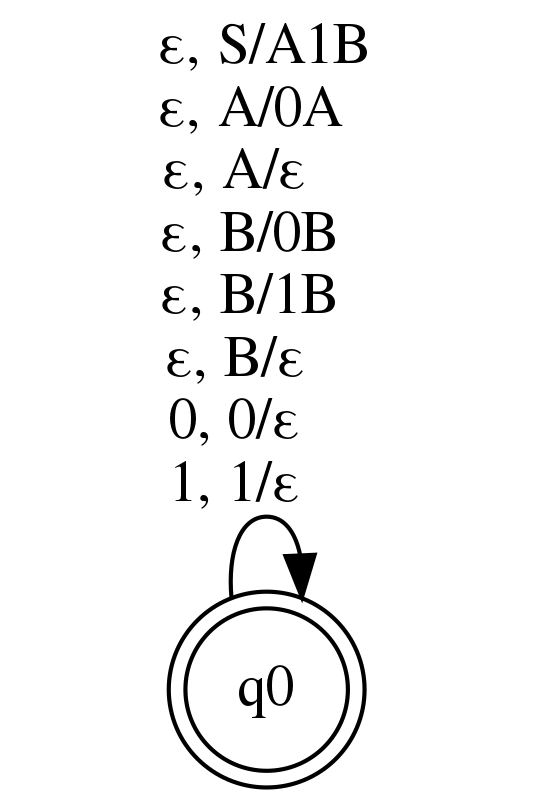
\includegraphics[scale=0.12]{PA08_1a}
\end{center}
\subsubsection{Item b}
\begin{center}
\begin{minipage}[c]{0.5\textwidth}
	\begin{alignat*}{2}
		PDA    &=  (Q, \Sigma, \Gamma, \delta, q_0, Z_0)\\
		Q      &= \{q_0\}\\
		\Sigma &= \{\text{0},\text{1}\}\\
		\Gamma &= \{\text{0},\text{1},\text{A},\text{B},\text{S}\}\\
		Z_0    &= \text{S}\\
		\delta &\colon Q \times (\Sigma \cup \{\varepsilon\} ) \times \Gamma \rightarrow \mathscr{P}(Q \times \Sigma^\ast)
	\end{alignat*}
\end{minipage}%
\begin{minipage}[c]{0.5\textwidth}
	\begin{alignat*}{2}
		&\delta(q_0, \varepsilon ,\text{S}&&) = \{(q_0, \text{A1B})\}\\
		&\delta(q_0, \varepsilon, \text{A}&&) = \{(q_0, \text{0A} ), (q_0,\varepsilon)\}\\
		&\delta(q_0, \varepsilon, \text{B}&&) = \{(q_0, \text{0B} ), (q_0, \text{1B}), (q_0,\varepsilon)\}\\
		\forall s \in \Sigma ,\, &\delta(q_0,s,s&&) = \{(q_0,\varepsilon)\}
	\end{alignat*}
\end{minipage}%
\end{center}
\subsubsection{Item c}
To trace the computations of the PDA, we will assume the top of the stack is on the left.
\begin{alignat*}{9}
	(q_0, \text{10}, \text{S})
	&\vdash (q_0, &\text{10}   &, &\text{A1B}  &)\\
	&\vdash (q_0, &\text{10}   &, &\text{1B}   &)\\
	&\vdash (q_0, &\text{0}    &, &\text{B}    &)\\
	&\vdash (q_0, &\text{0}    &, &\text{0B}   &)\\
	&\vdash (q_0, &\varepsilon &, &\text{B}    &)\\
	&\vdash (q_0, &\varepsilon &, &\varepsilon &)
\end{alignat*}
\subsubsection{Item d}
This PDA is non-deterministic, given there is at least one triple $(q,a,t) \in Q \times (\Sigma \cup \{\varepsilon\} ) \times \Gamma $ such that $\#\delta(q,a,t) > 1$. This is true given we can present the case $(q_0,\varepsilon,\text{A})$, that maps to either $(q_0,\text{0A})$ or $(q_0,\varepsilon)$.
}